\documentclass[a4paper,11pt]{article}
\usepackage{fullpage}
\usepackage[latin1]{inputenc}
\usepackage[T1]{fontenc}
\usepackage[normalem]{ulem}
\usepackage[english]{babel}
\usepackage{listings,babel}
\lstset{breaklines=true,basicstyle=\ttfamily}
\usepackage{graphicx}
\usepackage{moreverb}
\usepackage{url}
\usepackage{amsmath}
\usepackage{float}
\usepackage{tabularx}

\title{Texture Mapping Unit, Revision 2}
\author{S\'ebastien Bourdeauducq}
\date{April 2010}
\begin{document}
\setlength{\parindent}{0pt}
\setlength{\parskip}{5pt}
\maketitle{}

\section{Presentation}
The texture mapping unit supports the following operations:
\begin{itemize}
\item 2D texture mapping on a tesselation of equally-sized rectangles.
\item Operates only on rectangular rendering primitives (no triangles).
\item Fixed-point texture coordinates (1/64 pixel resolution).
\item Configurable bilinear texture filtering.
\item Configurable texture wrapping (only dimensions that are a power of 2 are supported for wrapping).
\item Configurable texture clamping (any dimension).
\item Up to 2047x2047 texture size.
\item Up to 2047x2047 output buffer resolution.
\item Chroma key filtering.
\item Fading to black.
\end{itemize}

The core processes 16-bit RGB565 progressive-scan framebuffers, accessed via FML links with a width of 64 bits and a burst length of 4.

The vertex data is fetched using a 32-bit WISHBONE master. Connecting this bus to the WISHBONE-to-FML caching bridge allows the mesh data to be stored in cost-effective DRAM.

For controlling the core, a CSR bus slave is also implemented.

\section{Configuration and Status Registers}
Registers can be read at any time, and written when the core is not busy. Write operations when the busy bit is set in register 0, including those to the control register, are illegal and can cause unpredictable behaviour.

Addresses are in bytes to match the addresses seen by the CPU when the CSR bus is bridged to Wishbone.

\subsection{Parameters and control}
\begin{tabularx}{\textwidth}{|l|l|l|X|}
\hline
\bf{Offset} & \bf{Access} & \bf{Default} & \bf{Description} \\
\hline
0x00 & RW & 0 & Control register. \\
& & & Bit 0: Start/Busy.\\
& & & Bit 1: Enable chroma key. \\
\hline
0x04 & RW & 32 & Number of mesh rectangles in the X direction (which is the number of mesh points minus one, and also the index of the last mesh point). \\
\hline
0x08 & RW & 24 & Number of mesh rectangles in the Y direction. \\
\hline
0x0C & RW & 63 & Brightness, between 0 and 63. The components of each pixel are multiplied by $ (n+1) \over 64 $ and rounded to the lowest integer. That means that a value of 0 in this register makes the destination picture completely black (because of the limited resolution of RGB565). \\
\hline
0x10 & RW & 0 & RGB565 color used as chroma key. Texture pixels with this color will not be drawn if the ``chroma key'' flag in the control register is set. \\
\hline
0x14 & RW & 0 & Vertex mesh address. The address must be aligned to a 64-bit boundary. \\
\hline
0x18 & RW & 0 & Texture buffer address. The address must be aligned to a 16-bit boundary. \\
\hline
0x1C & RW & 512 & Texture horizontal resolution. \\
\hline
0x20 & RW & 512 & Texture vertical resolution. \\
\hline
0x24 & RW & 0x3ffff & Binary mask ANDed to the fixed-point X texture coordinate during interpolation. This mask can be used to control texture wrapping and filtering. \\
\hline
0x28 & RW & 0x3ffff & Binary mask ANDed to the fixed-point Y texture coordinate during interpolation. \\
\hline
0x2C & RW & 0 & Destination framebuffer address. The address be aligned to a 16-bit boundary. \\
\hline
0x30 & RW & 640 & Destination horizontal resolution. \\
\hline
0x34 & RW & 480 & Destination vertical resolution. \\
\hline
0x38 & RW & 0 & X offset added to each destination pixel, allowing the use of the TMU as a blitter. Negative offsets in two's complement format are supported. \\
\hline
0x3C & RW & 0 & Y offset added to each destination pixel. \\
\hline
0x40 & RW & 16 & Width of each destination rectangle. \\
\hline
0x44 & RW & 16 & Height of each destination rectangle. \\
\hline
0x48 & RW & 63 & Opacity (alpha) used when drawing in the destination framebuffer. 0 = high transparency, 63 = totally opaque. A value of 63 saves memory bandwidth by removing the need to read-modify-write the destination framebuffer. \\
\hline
\end{tabularx}

\section{Interrupts}
The TMU is equipped with one active-high edge-sensitive interrupt line.

An interrupt is triggered when a texture mapping is done and all resulting data has been sent through the bus master.

\section{Encoding the vertex data}
The core supports a maximum mesh of 128x128 points. The address of the point at indices $ (x, y) $ in the mesh is, regardless of the actual the number of mesh points:

\begin{equation*}
base + 8 \cdot (128 \cdot y + x)
\end{equation*}

This means that the mesh always has the same size in memory.

Each point is made up of 64 bits, with the 32 upper bits being the X coordinate and the 32 lower bits the Y coordinate, in fixed-point two's complement signed format with 6 bits of fractional part.

Exactly 128kB are used by the mesh.

\section{Architecture}

The texture mapping unit has a deeply pipelined architecture following the ``dataflow'' model. The first stage fetches vertex data, which are in turn passed to the second stage which computes operands for the division, done in the third stage, used in linear interpolations, etc.

\subsection{Handshake protocol between pipeline stages}
Because pipeline stages are not always ready to accept and/or to produce data (because, for example, of memory latencies), a flow control protocol must be implemented.

The situation is the same between all stages: an upstream stage is registering data into a downstream stage. During some cycles, the upstream stage cannot produce valid data and/or the downstream stage is processing the previous data and has no memory left to store the incoming data.

\begin{figure}[H]
\centering
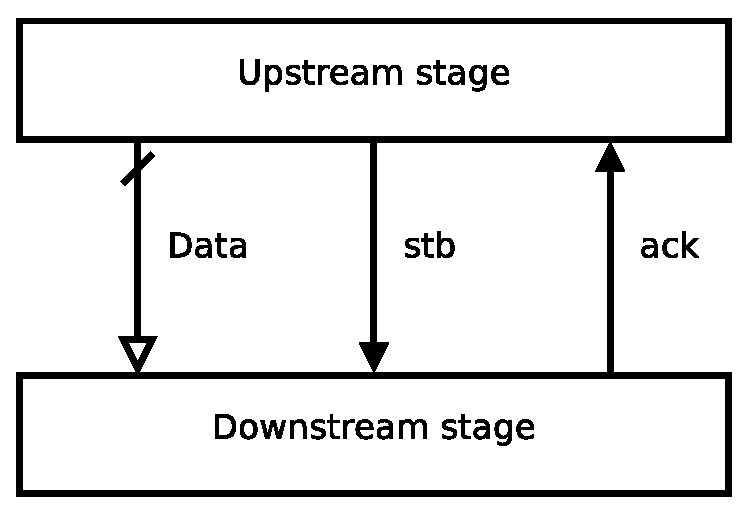
\includegraphics[height=30mm]{comm.eps}
\caption{Communication between two pipeline stages.}\label{fig:comm}
\end{figure}

Appropriate handling of these cases is done using standardized \verb!stb! and \verb!ack! signals. The meaning of these is summarized in this table:\\

\begin{tabularx}{\textwidth}{|l|l|X|}
\hline
\bf stb & \bf ack & \bf Situation \\
\hline
0 & 0 & The upstream stage does not have data to send, and the downstream stage is not ready to accept data. \\
\hline
0 & 1 & The downstream stage is ready to accept data, but the upstream stage has currently no data to send. The downstream stage is not required to keep its ack signal asserted. \\
\hline
1 & 0 & The upstream stage is trying to send data to the downstream stage, which is currently not ready to accept it. The transaction is \textit{stalled}. The upstream stage must keep stb asserted and continue to present valid data until the transaction is completed. \\
\hline
1 & 1 & The upstream stage is sending data to the downstream stage which is ready to accept it. The transaction is \textit{completed}. The downstream stage must register the incoming data, as the upstream stage is not required to hold it valid at the next cycle. \\
\hline
\end{tabularx}\\

It is not allowed to generate \verb!ack! combinatorially from \verb!stb!. The \verb!ack! signal must always represent the current state of the downstream stage, ie. whether or not it will accept whatever data we present to it.

\section{Bilinear filtering}
\subsection{Principle}
Bilinear filtering works by adding 6 extra bits of precision to the texture coordinates, which become fixed-point non-integer coordinates.

Those bits are used to compute a weighted average of 4 neighbouring texture pixels when the interpolated texture coordinates are not integer.

\begin{figure}[H]
\centering
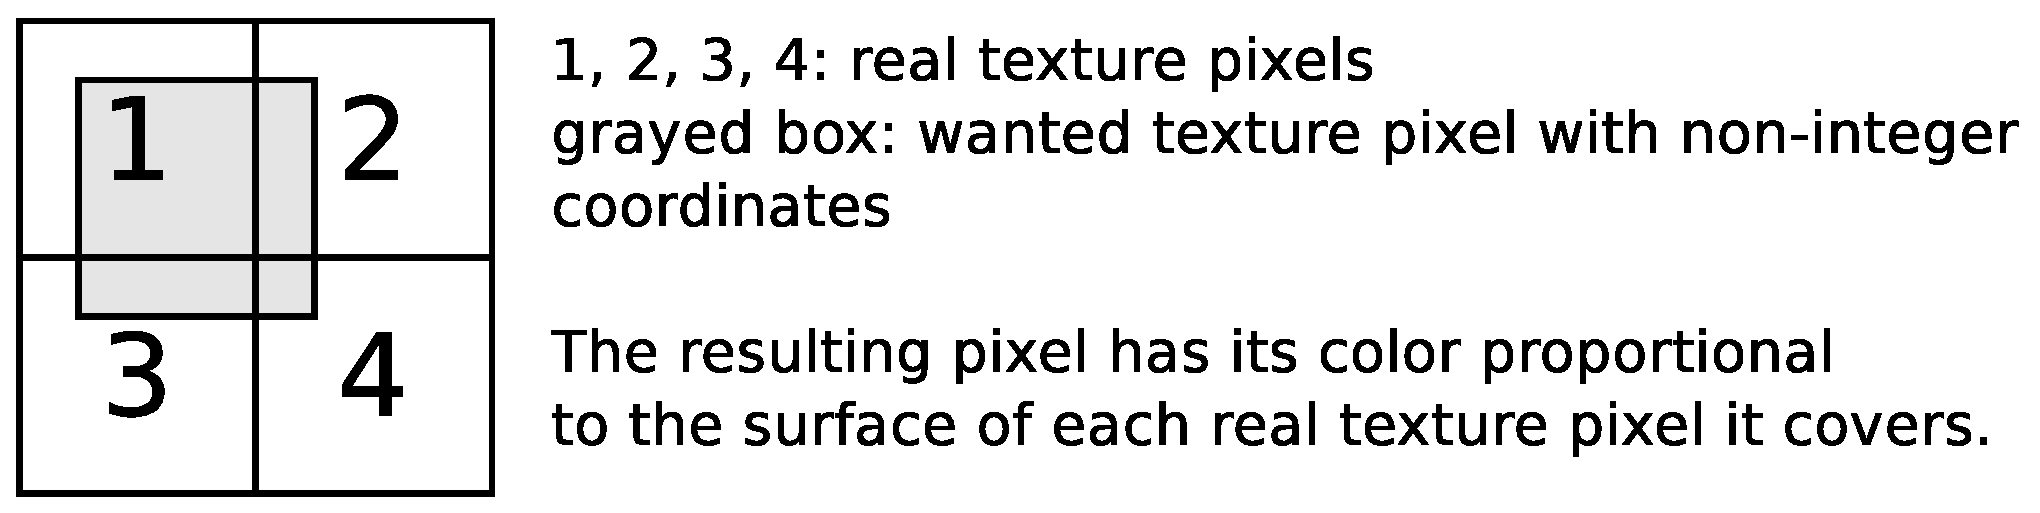
\includegraphics[height=32mm]{bilinear.eps}
\caption{Principle of bilinear texture filtering.}\label{fig:bilinear}
\end{figure}

\subsection{Pixel distribution in the cache}
Because of performance requirements, all four texture pixels must be fetched in one clock cycle. It is therefore relevant to examine their distribution in the cache, to determine what cache architecture should be used.

\subsubsection{General case, middle of texture}
\begin{figure}[H]
\centering
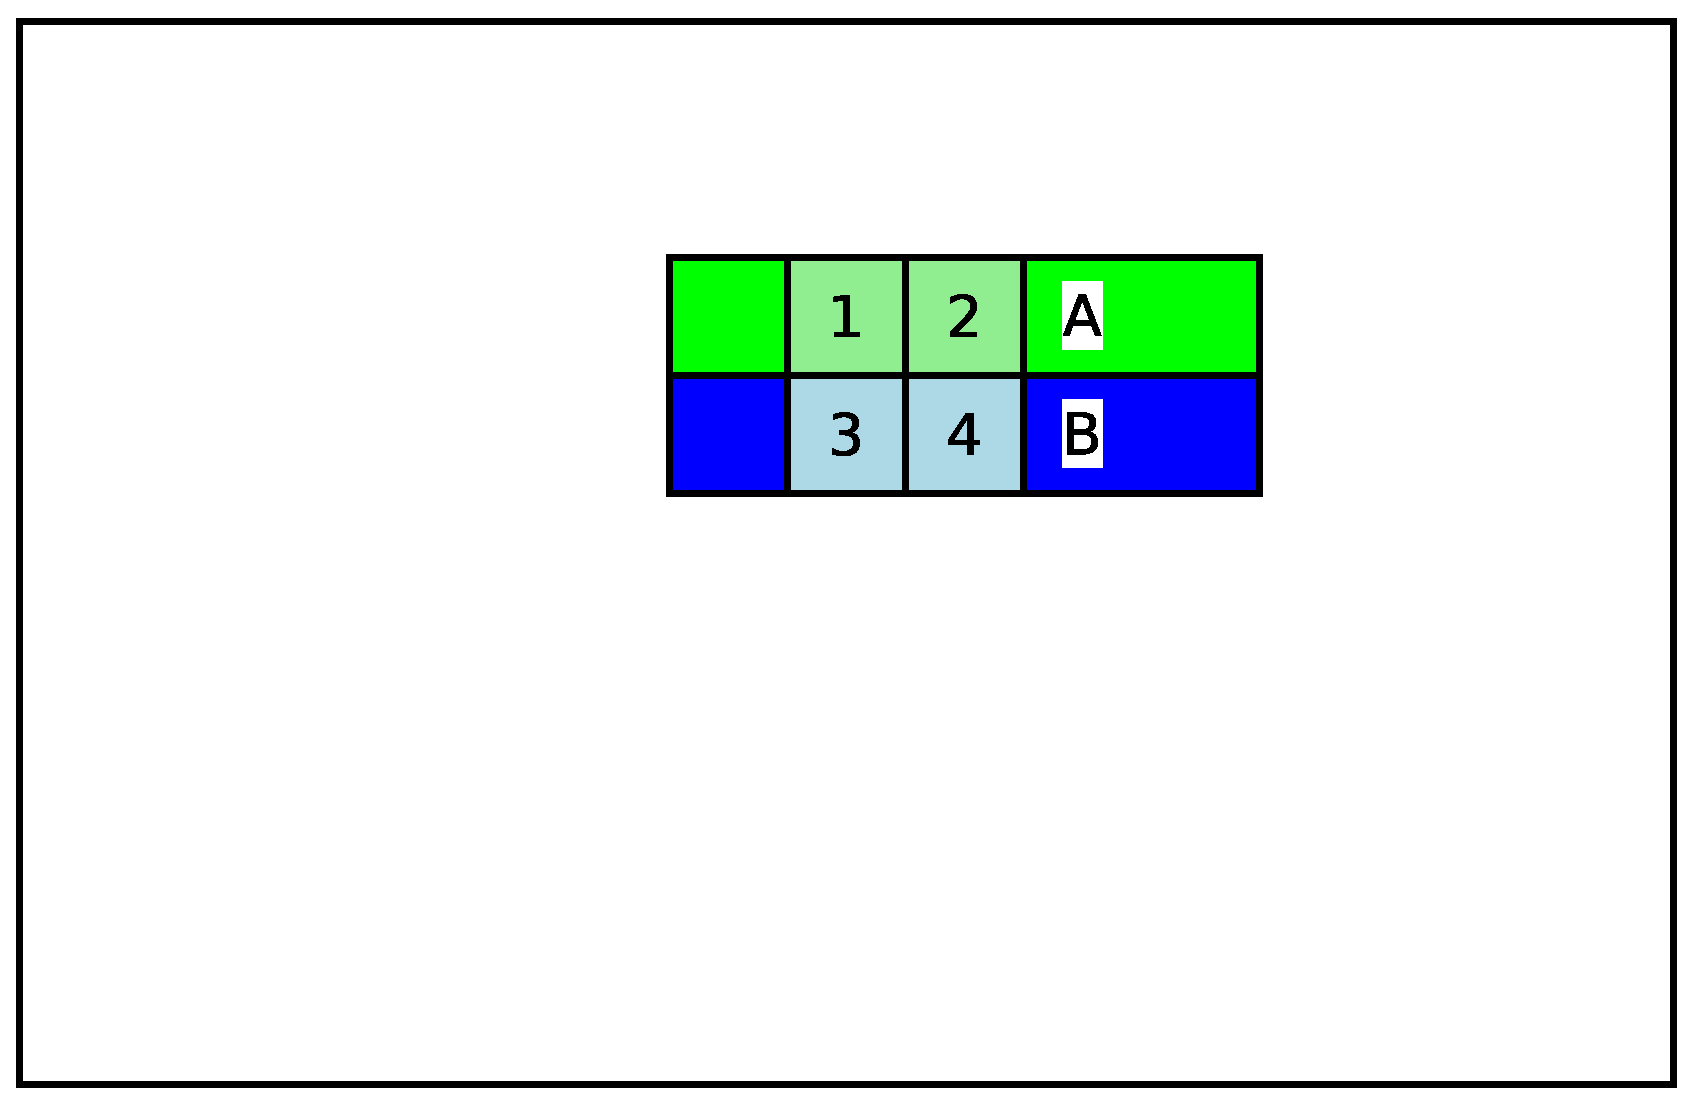
\includegraphics[height=55mm]{dist_common.eps}
\caption{Most common case, pixels 1 and 2 are in the same cache line.}\label{fig:case1}
\end{figure}

\begin{figure}[H]
\centering
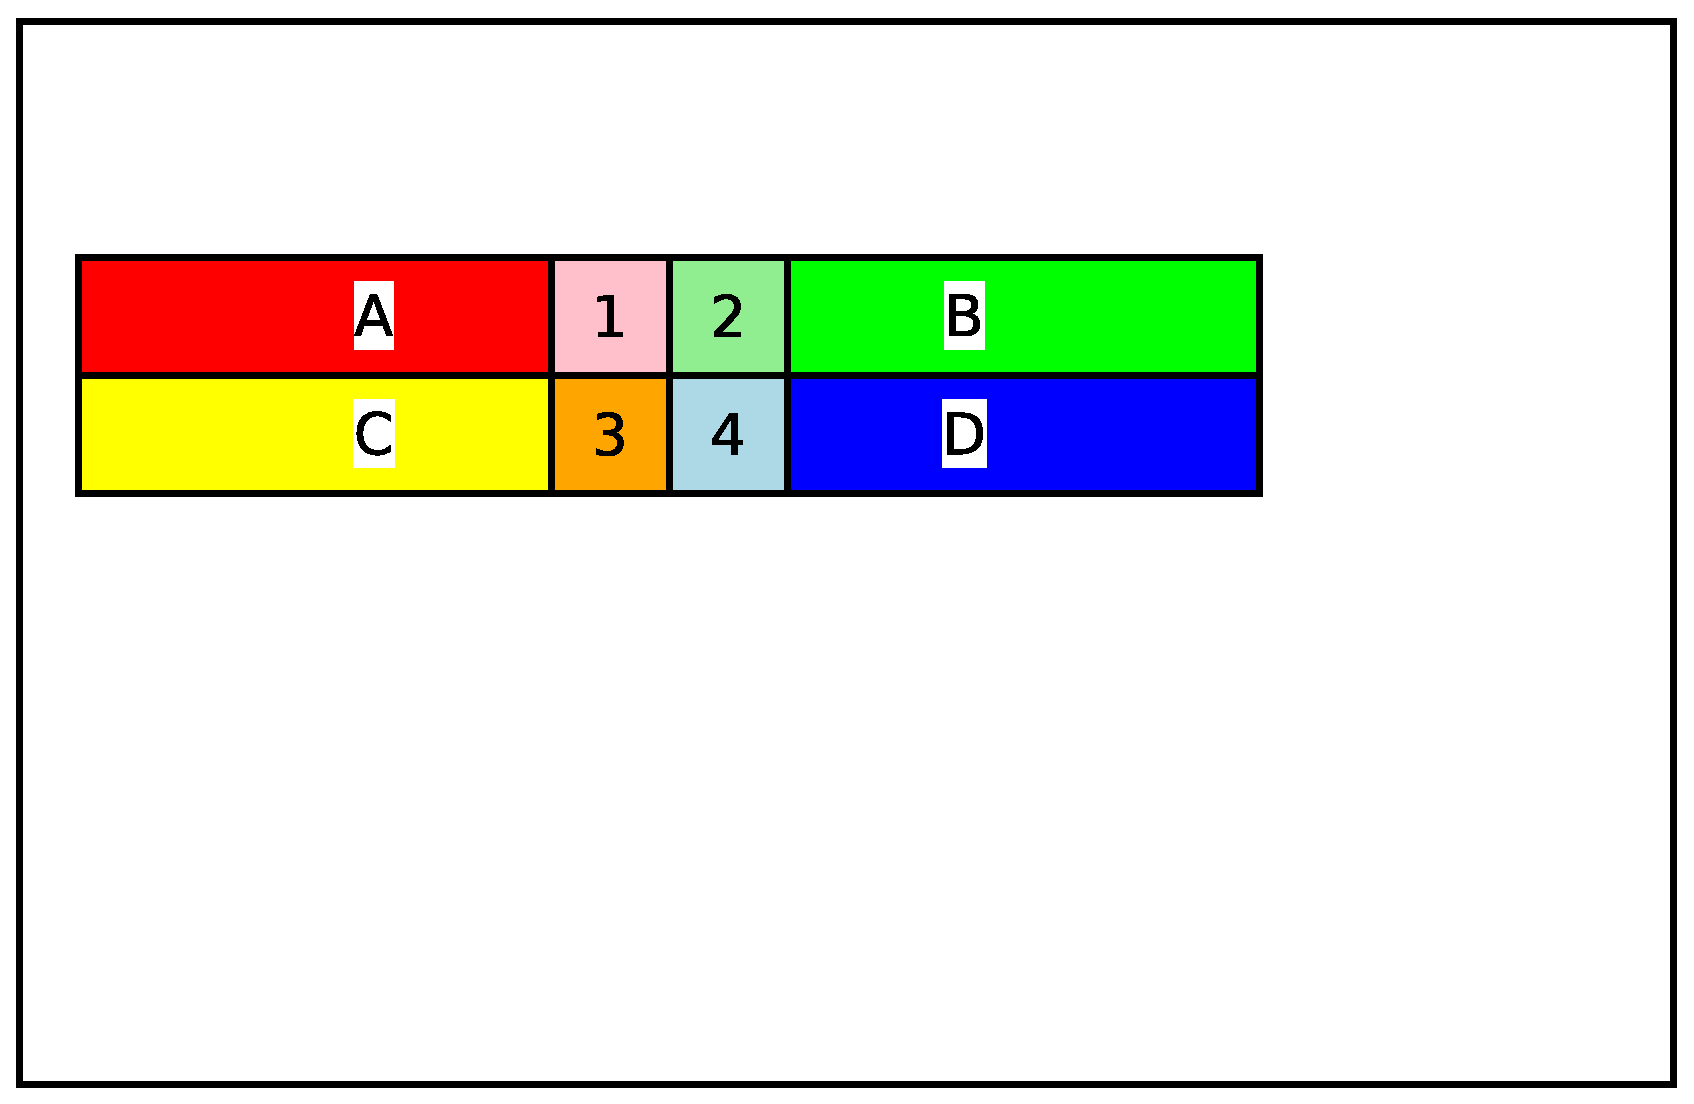
\includegraphics[height=55mm]{dist_12lines.eps}
\caption{Pixels 1 and 2 are in different cache lines.}\label{fig:case2}
\end{figure}

\subsubsection{With clamping}
When pixels go out of the texture, clamping can induce cases where two or four pixels merge.

\begin{figure}[H]
\centering
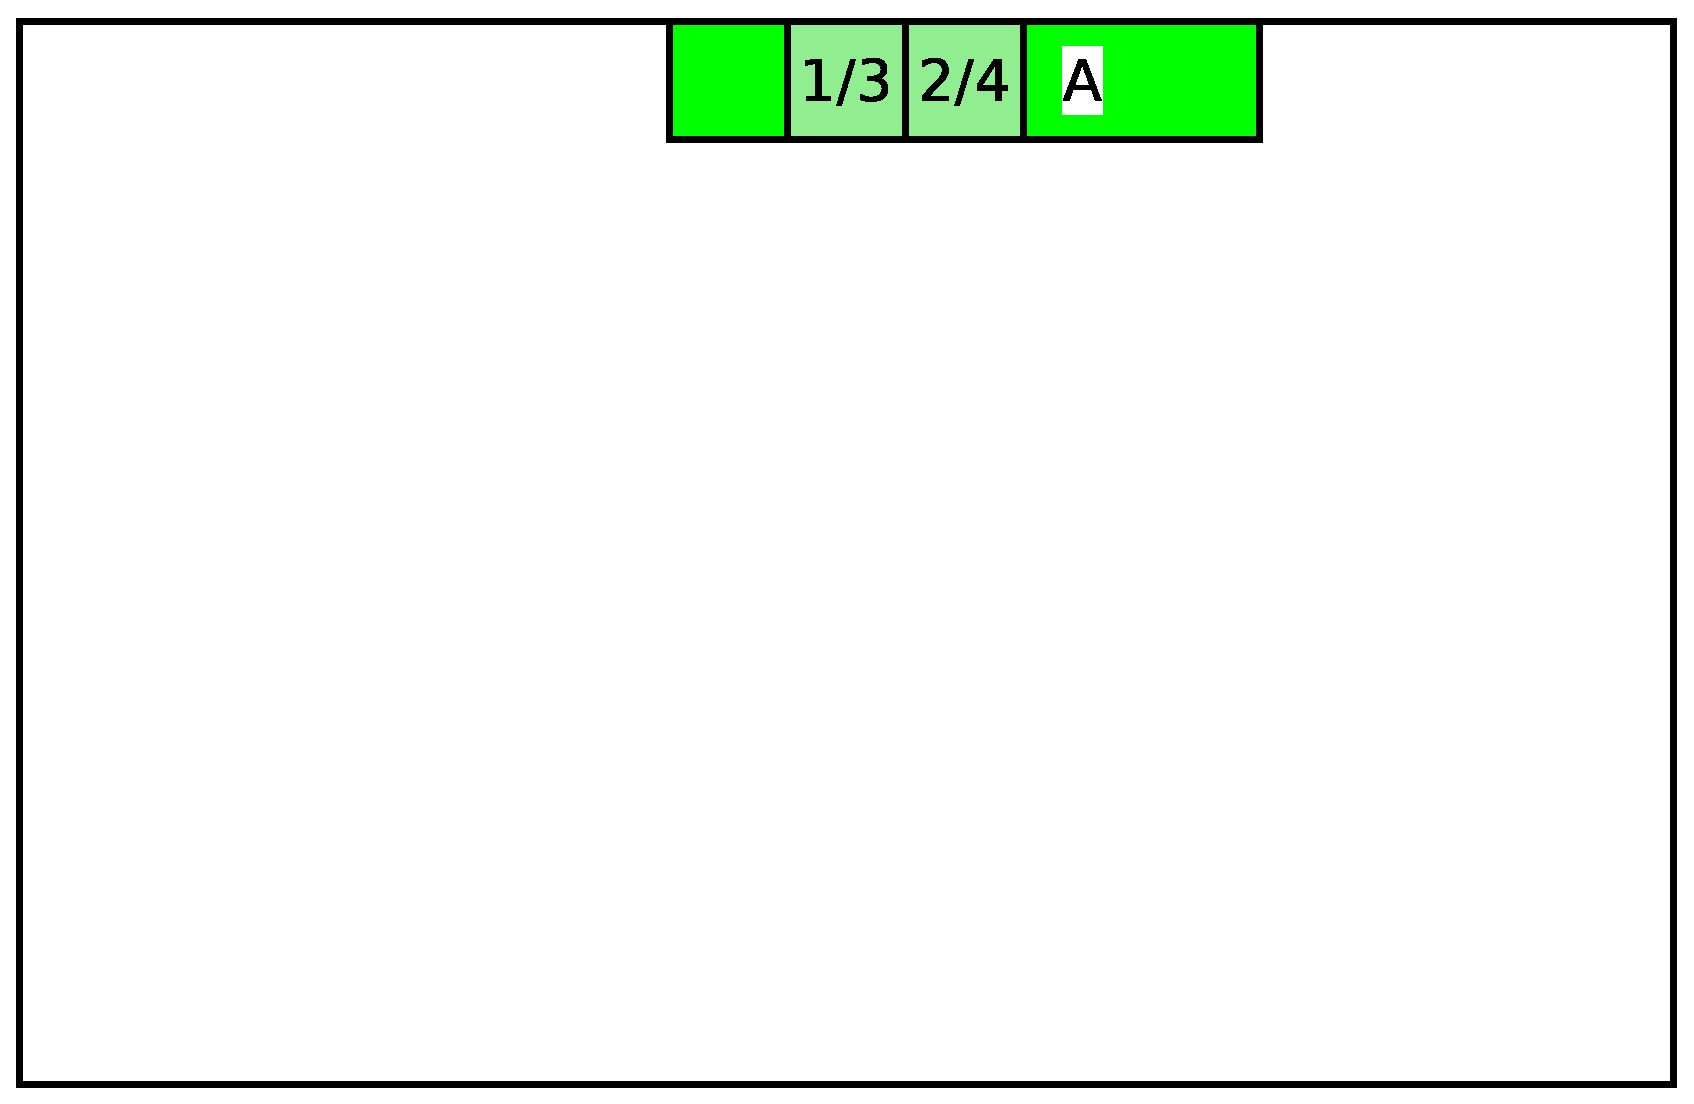
\includegraphics[height=55mm]{dist_clamp.eps}
\caption{Example of pixels merging because Y1=-1.}\label{fig:caseclamp}
\end{figure}

\subsubsection{With wrapping}
Wrapping can cause pixels split across the texture. This can happen horizontally, vertically or both.

\begin{figure}[H]
\centering
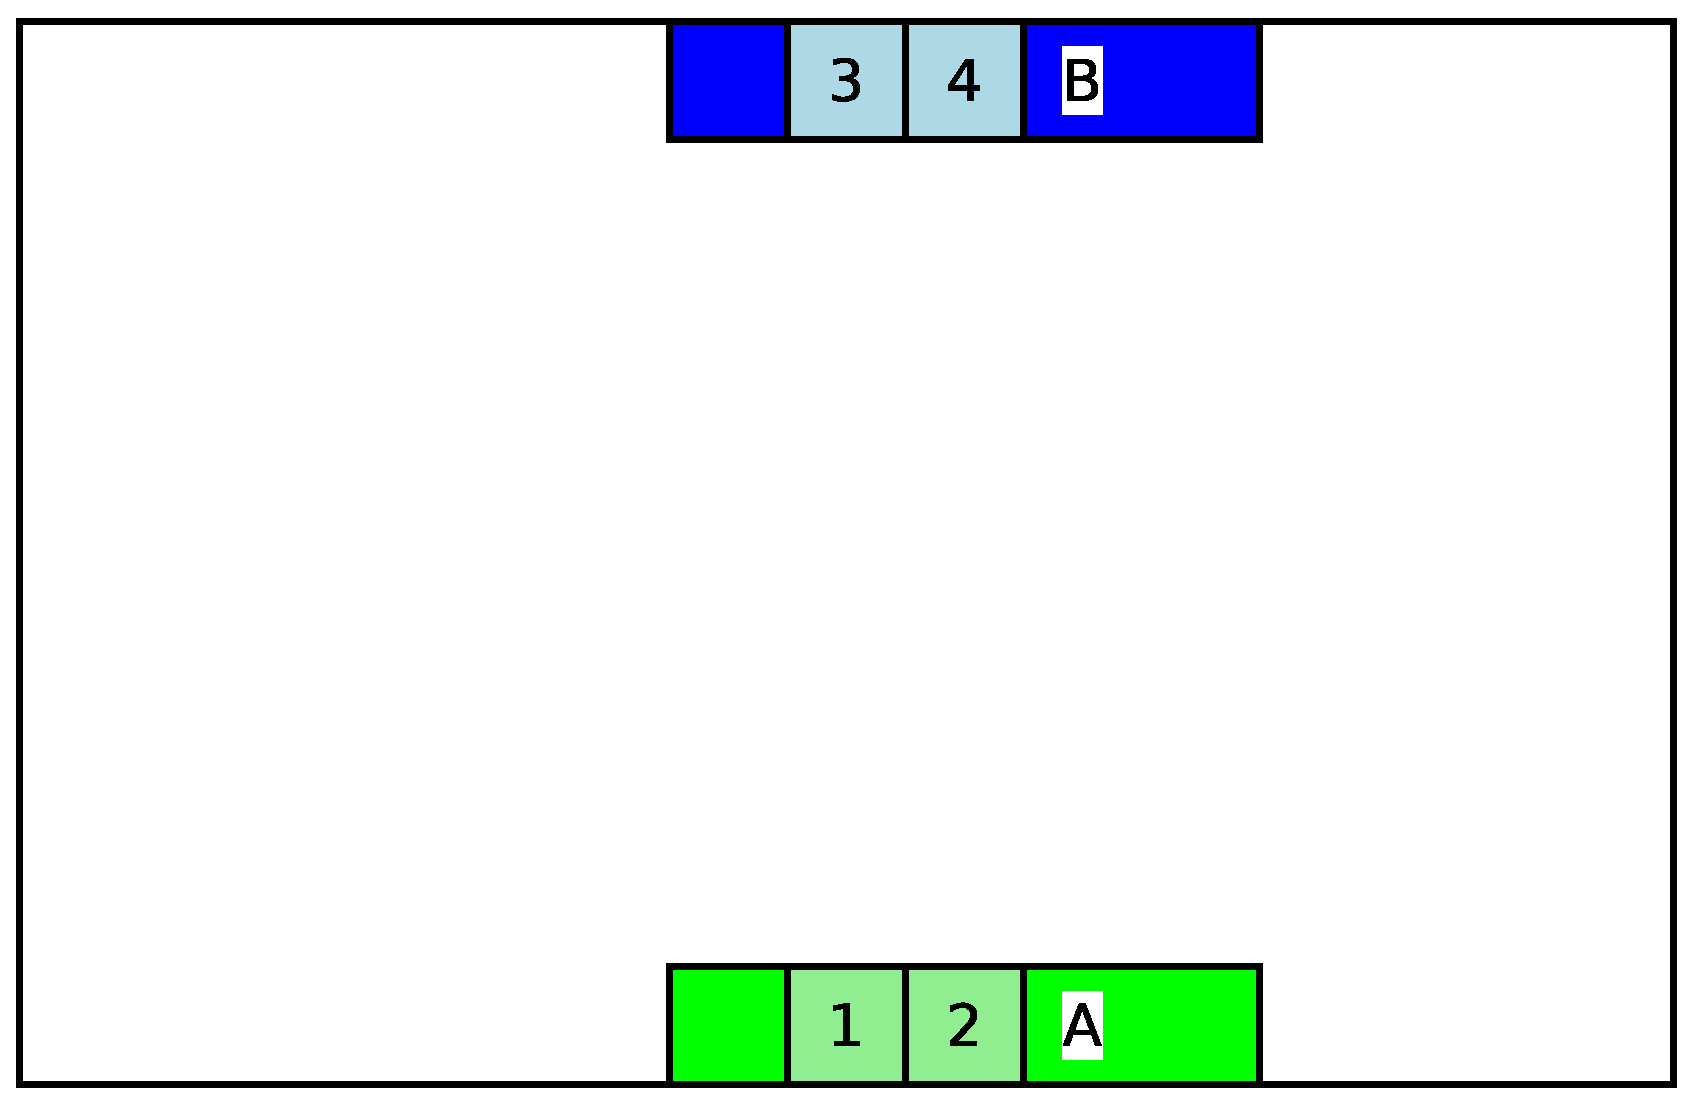
\includegraphics[height=55mm]{dist_wrap1.eps}
\caption{Vertical wrapping.}\label{fig:casewrap1}
\end{figure}

\begin{figure}[H]
\centering
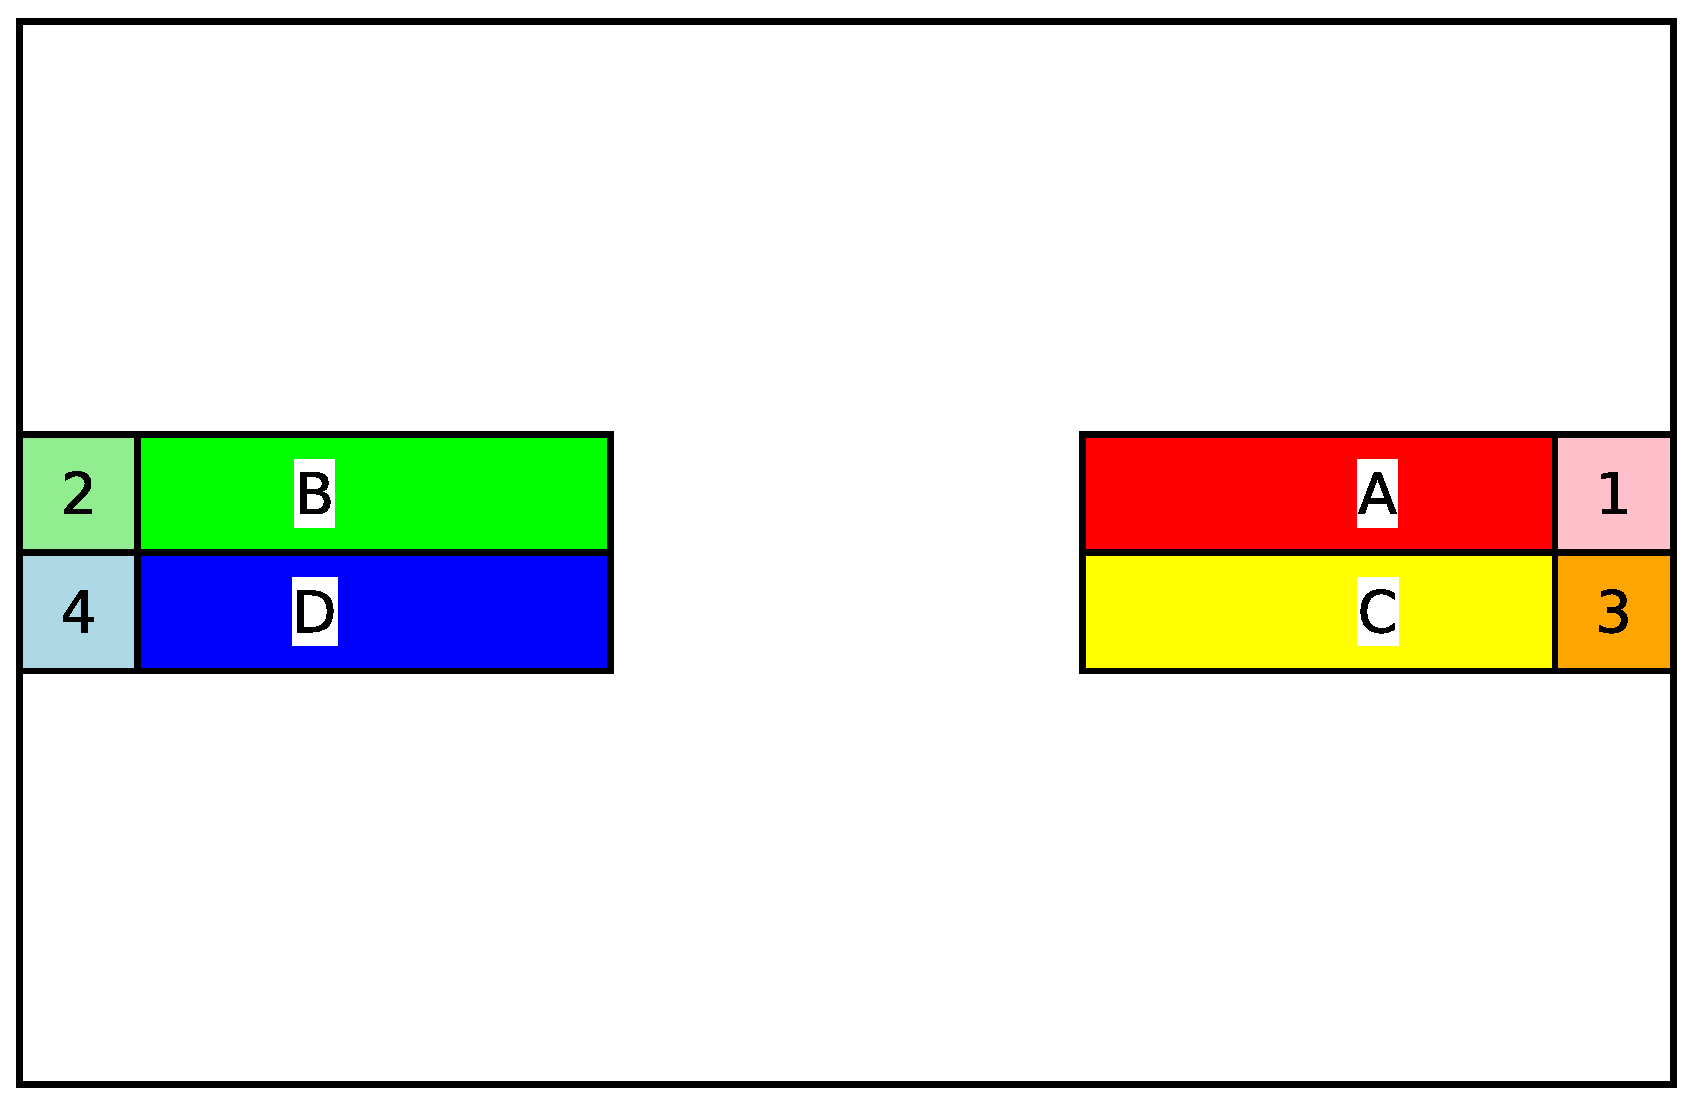
\includegraphics[height=55mm]{dist_wrap2.eps}
\caption{Horizontal wrapping.}\label{fig:casewrap2}
\end{figure}

\begin{figure}[H]
\centering
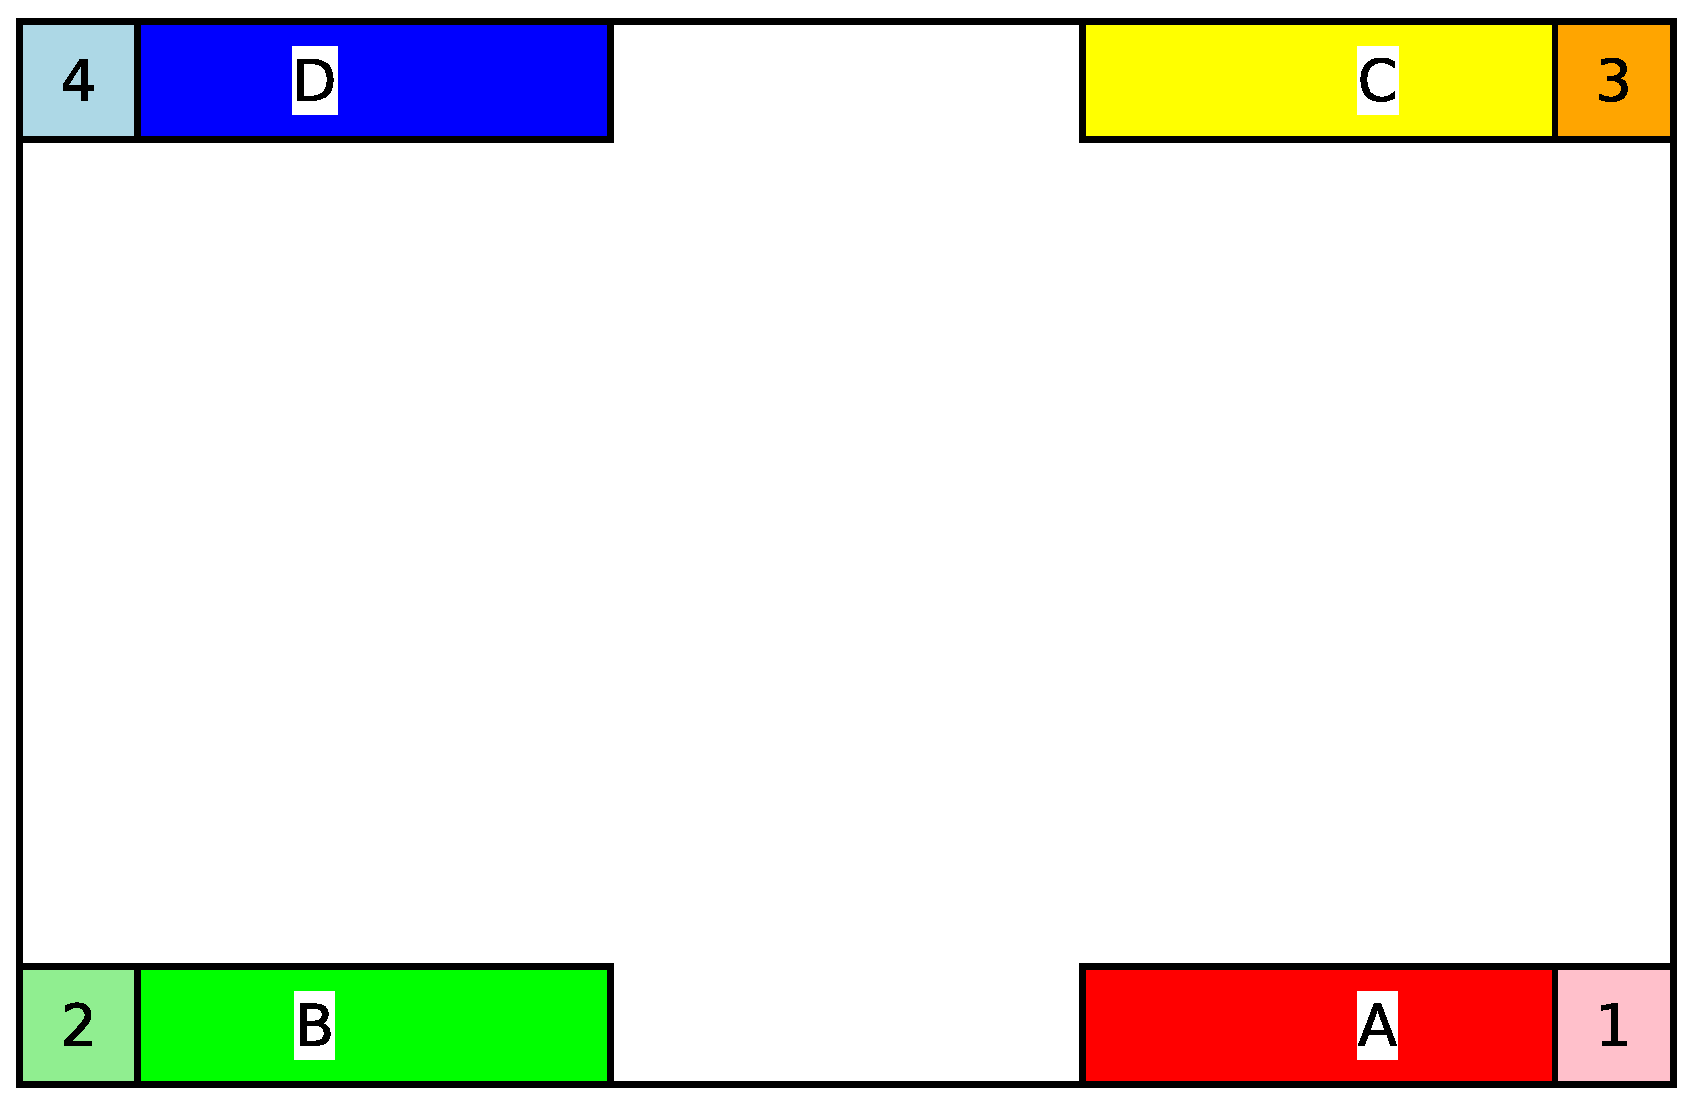
\includegraphics[height=55mm]{dist_wrap3.eps}
\caption{Wrapping in both directions.}\label{fig:casewrap3}
\end{figure}

\subsection{Cache architecture}
\subsubsection{Design options}
We have two options for designing the cache:
\begin{itemize}
\item four separate caches (one for pixel 1, one for pixel 2, etc.)
\item a shared cache capable of looking up 4 pixels at a time
\end{itemize}

Misses happening in the ways for pixels 1, 2, 3 and 4 are likely to be correlated, so a shared cache architecture is chosen to minimize memory bandwidth.

\subsubsection{Avoiding cache conflicts}
There could be replacement conflicts that have, at least, a detrimental impact of performance.

Such conflicts happen when:
\begin{itemize}
\item (Figure~\ref{fig:case1}) lines A and B collide. This happens when:
\begin{equation*}
\text{hres} \equiv 0 \pmod{\text{csize}}
\end{equation*}
\item (Figure~\ref{fig:case2}) lines A and B collide or lines C and D collide. This does not happen unless the cache only contains one line, which is not a practical case.
\item (Figure~\ref{fig:case2}) lines A and C or lines B and D collide. This is the same case as for Figure~\ref{fig:case1}.
\item (Figure~\ref{fig:casewrap1}) lines A and B collide. This happens when:
\begin{equation*}
\text{hres}\cdot(\text{vres}-1) \equiv 0 \pmod{\text{csize}}
\end{equation*}
\item (Figure~\ref{fig:casewrap2}) lines A and B or lines B and C collide. This happens when:
\begin{equation*}
\text{hres}-1 \equiv 0 \pmod{\text{csize}}
\end{equation*}
\end{itemize}

In the equations above:
\begin{itemize}
\item hres is the horizontal resolution in pixels
\item vres is the vertical resolution in pixels
\item csize is the total number of pixels the cache can hold. It is equal to the cache size in bytes (not counting the tag memory) divided by 2.
\end{itemize}

\subsubsection{Chosen architecture}
The block diagram of the cache architecture is given in Figure~\ref{fig:carch}.

\begin{figure}[H]
\centering
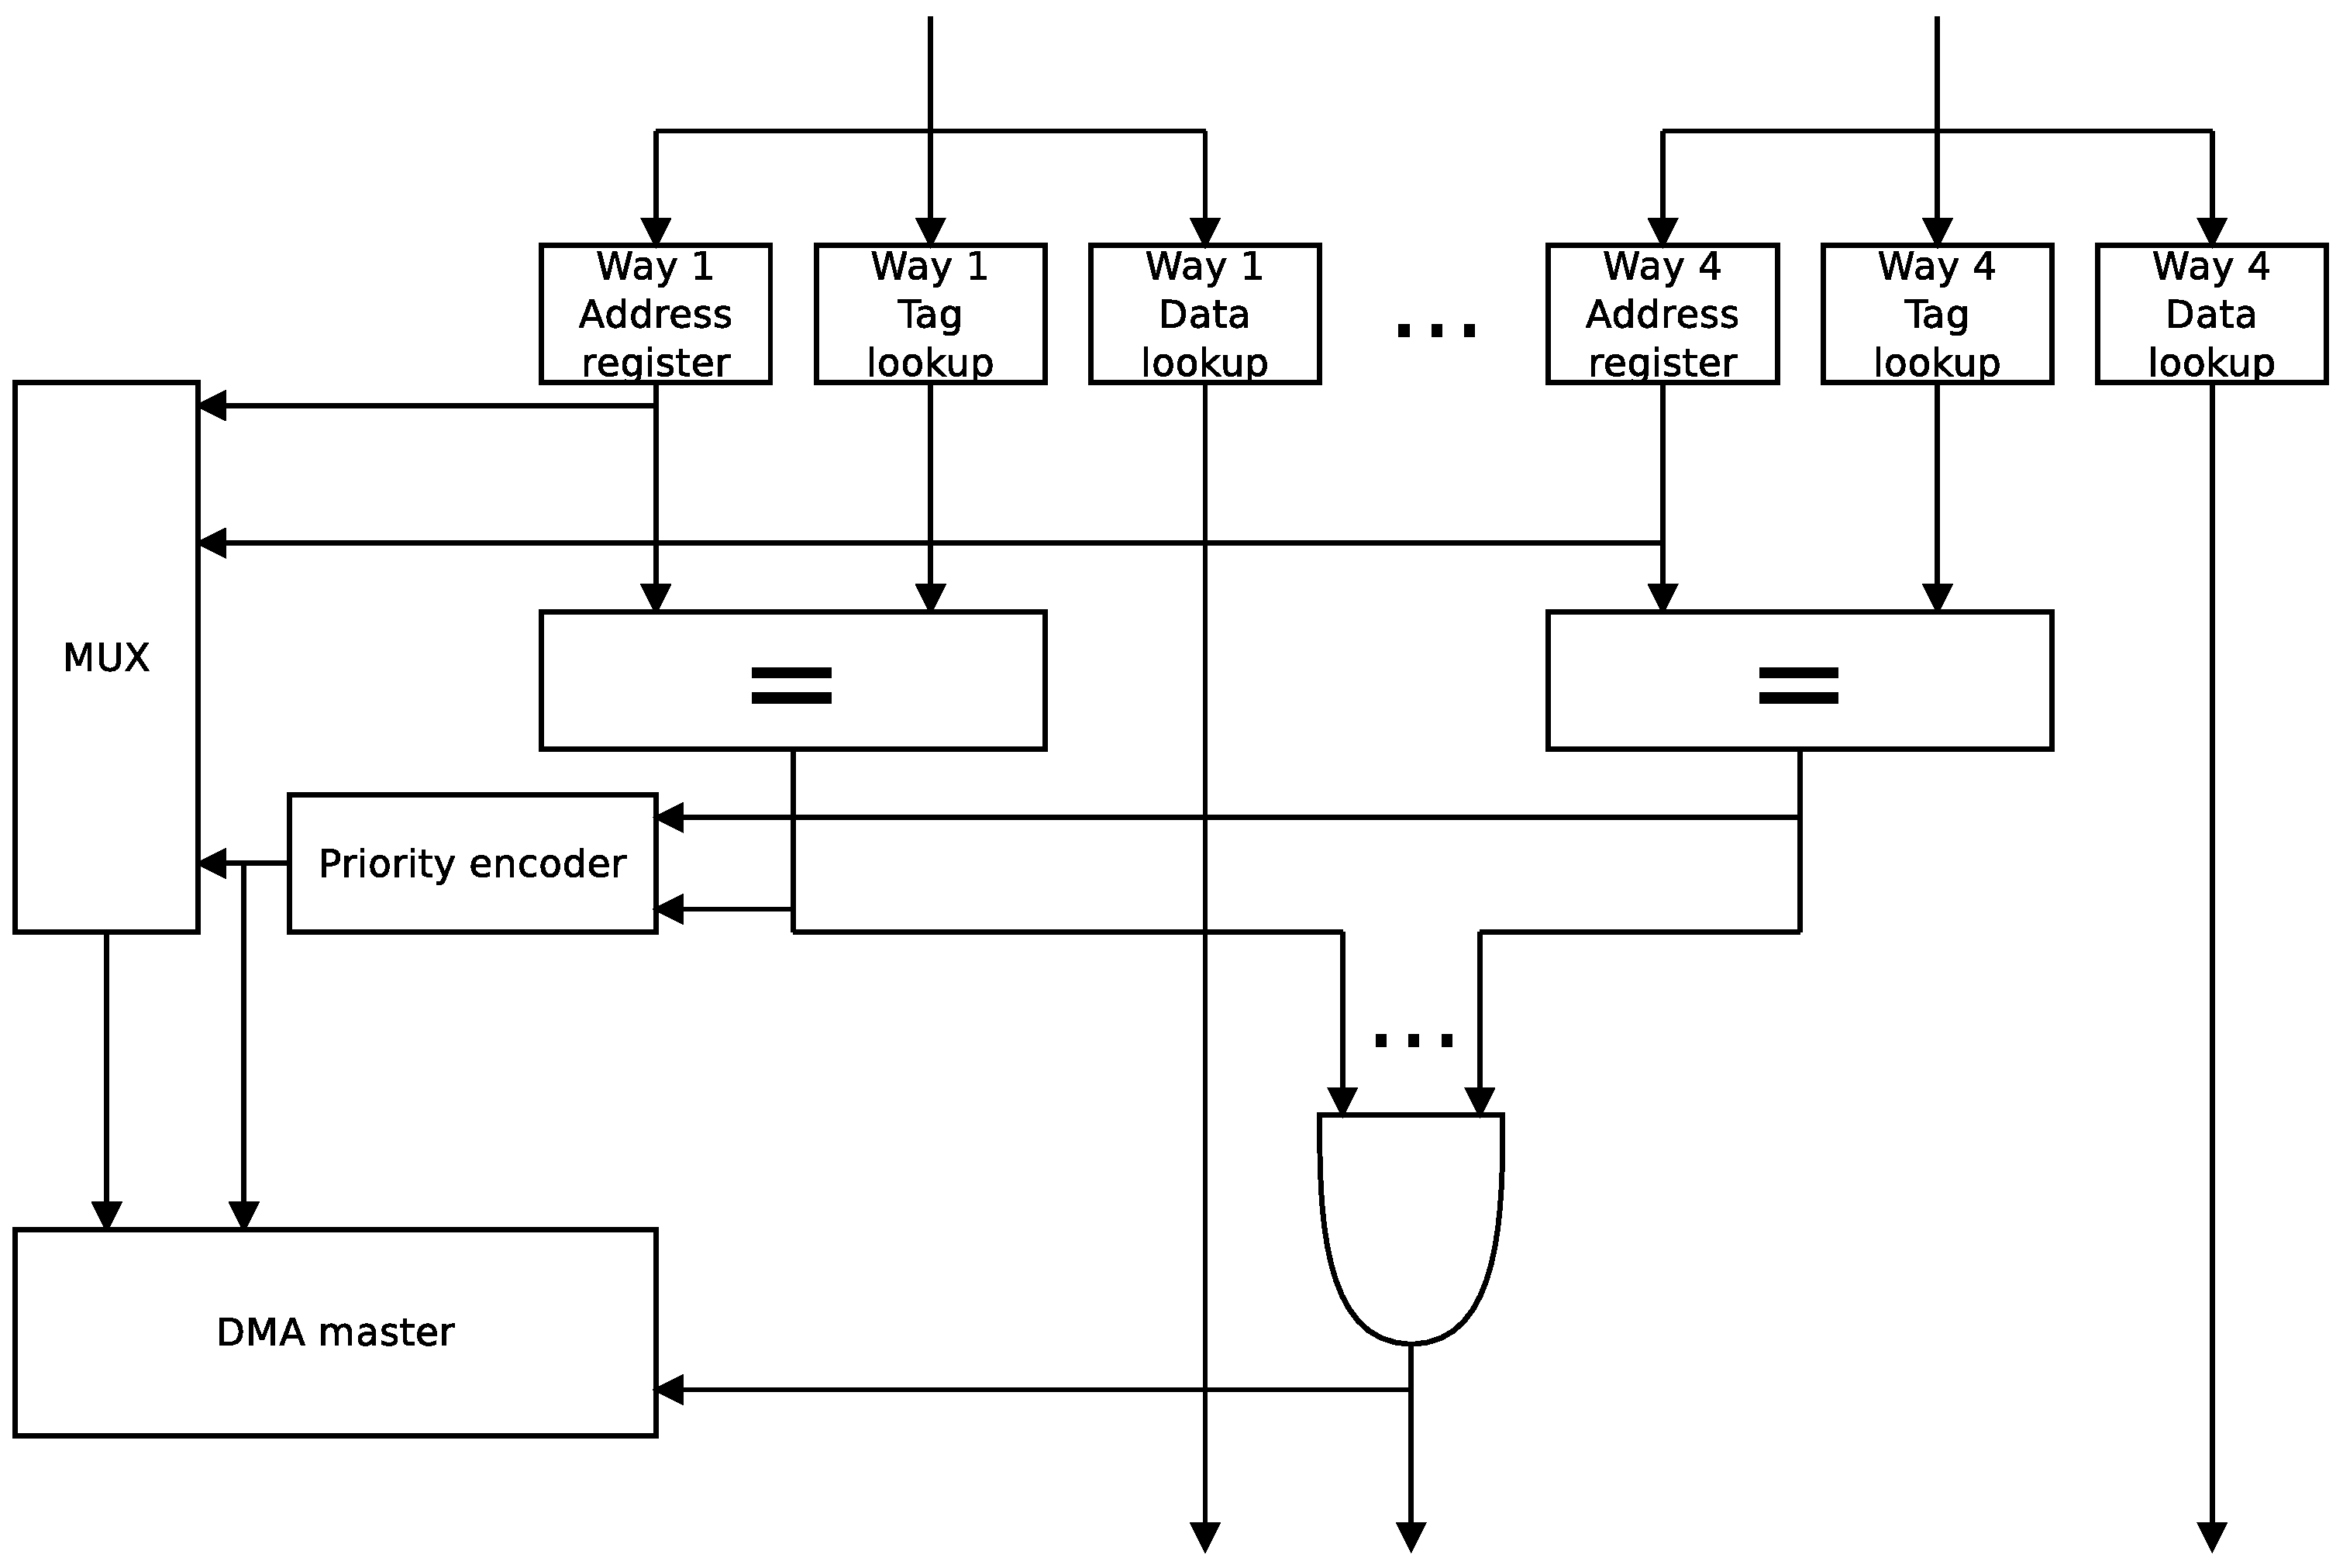
\includegraphics[height=95mm]{carch.eps}
\caption{TMU cache architecture for bilinear filtering.}\label{fig:carch}
\end{figure}

Because cache conflicts can be easily be avoided by choosing the texture resolution carefully, they are not handled by this architecture. \textbf{Having a cache conflict results in a lockup of the cache controller}, that requires a reset of the core.

The four-way cache can be efficently implemented on FPGA targets by using two dual-port block RAMs.

\subsubsection{Summary}
In order to avoid cache conflicts which lock up the core, one must make sure that:
\begin{equation*}
\text{hres} \not \equiv 0 \pmod{\text{csize}}
\end{equation*}
Additionally, if texture wrapping is enabled, one must also make sure that:
\begin{equation*}
\text{hres}\cdot(\text{vres}-1) \not \equiv 0 \pmod{\text{csize}}
\end{equation*}
\begin{equation*}
\text{hres}-1 \not \equiv 0 \pmod{\text{csize}}
\end{equation*}

\section*{Copyright notice}
Copyright \copyright 2007-2010 S\'ebastien Bourdeauducq. \\
Permission is granted to copy, distribute and/or modify this document under the terms of the GNU Free Documentation License, Version 1.3; with no Invariant Sections, no Front-Cover Texts, and no Back-Cover Texts. A copy of the license is included in the LICENSE.FDL file at the root of the Milkymist source distribution.

\end{document}
